\documentclass[12pt]{article}
\usepackage{fontspec}
\usepackage{fullpage}
\usepackage{hyperref}
\hypersetup{bookmarks=true,colorlinks=true,linkcolor=red,citecolor=blue,filecolor=magenta,urlcolor=cyan}
\usepackage{amsmath}
\usepackage{amssymb}
\usepackage{mathtools}
\usepackage{unicode-math}
\usepackage{tabu}
\usepackage{longtable}
\usepackage{booktabs}
\usepackage{caption}
\usepackage{enumitem}
\usepackage{graphics}
\usepackage{filecontents}
\usepackage[backend=bibtex]{biblatex}
\usepackage{url}
\setmathfont{Latin Modern Math}
\newcommand{\gt}{\ensuremath >}
\newcommand{\lt}{\ensuremath <}
\global\tabulinesep=1mm
\newlist{symbDescription}{description}{1}
\setlist[symbDescription]{noitemsep, topsep=0pt, parsep=0pt, partopsep=0pt}
\bibliography{bibfile}
\title{Software Requirements Specification for Pendulum}
\author{Olu Owojaiye}
\begin{document}
\maketitle
\tableofcontents
\newpage
\section{Reference Material}
\label{Sec:RefMat}
This section records information for easy reference.

\subsection{Table of Units}
\label{Sec:ToU}
The unit system used throughout is SI (Système International d'Unités). In addition to the basic units, several derived units are also used. For each unit, \hyperref[Table:ToU]{Tab: ToU} lists the symbol, a description and the SI name.

\begin{longtable}{l l l}
\toprule
\textbf{Symbol} & \textbf{Description} & \textbf{SI Name}
\\
\midrule
\endhead
${{}^{\circ}}$ & angle & degree
\\
${\text{kg}}$ & mass & kilogram
\\
${\text{m}}$ & length & metre
\\
${\text{N}}$ & force & newton
\\
${\text{rad}}$ & angle & radian
\\
${\text{s}}$ & time & second
\\
\bottomrule
\caption{Table of Units}
\label{Table:ToU}
\end{longtable}
\subsection{Table of Symbols}
\label{Sec:ToS}
The symbols used in this document are summarized in \hyperref[Table:ToS]{Tab: ToS} along with their units. Throughout the document, symbols in bold will represent vectors, and scalars otherwise. The symbols are listed in alphabetical order. For vector quantities, the units shown are for each component of the vector.

\begin{longtable}{l l l}
\toprule
\textbf{Symbol} & \textbf{Description} & \textbf{Units}
\\
\midrule
\endhead
${a_{\text{x}}}$ & $x$-component of acceleration & $\frac{\text{m}}{\text{s}^{2}}$
\\
${a_{\text{y}}}$ & $y$-component of acceleration & $\frac{\text{m}}{\text{s}^{2}}$
\\
$\mathbf{a}$ & Acceleration & $\frac{\text{m}}{\text{s}^{2}}$
\\
$\mathbf{F}$ & Force & ${\text{N}}$
\\
${L_{\text{rod}}}$ & Length of rod & ${\text{m}}$
\\
$m$ & Mass & ${\text{kg}}$
\\
${{p_{\text{x}}}^{\text{i}}}$ & $x$-component of initial position & ${\text{m}}$
\\
${{p_{\text{y}}}^{\text{i}}}$ & $y$-component of initial position & ${\text{m}}$
\\
$\mathbf{p}$ & Position & ${\text{m}}$
\\
$t$ & Time & ${\text{s}}$
\\
${v_{\text{x}}}$ & $x$-component of velocity & $\frac{\text{m}}{\text{s}}$
\\
${v_{\text{y}}}$ & $y$-component of velocity & $\frac{\text{m}}{\text{s}}$
\\
$\mathbf{v}$ & Velocity & $\frac{\text{m}}{\text{s}}$
\\
$α$ & Angular Acceleration & $\frac{\text{rad}}{\text{s}^{2}}$
\\
$θ$ & Angle of pendulum & ${{}^{\circ}}$
\\
$ω$ & Angular Velocity & $\frac{\text{rad}}{\text{s}}$
\\
\bottomrule
\caption{Table of Symbols}
\label{Table:ToS}
\end{longtable}
\subsection{Abbreviations and Acronyms}
\label{Sec:TAbbAcc}
\begin{longtable}{l l}
\toprule
\textbf{Abbreviation} & \textbf{Full Form}
\\
\midrule
\endhead
\bottomrule
\caption{Abbreviations and Acronyms}
\label{Table:TAbbAcc}
\end{longtable}
\section{Introduction}
\label{Sec:Intro}
pendulumTitle is the subject pendulumTitle is the focus. Pendulum.

The following section provides an overview of the Software Requirements Specification (SRS) for Pendulum. This section explains the purpose of this document, the scope of the requirements, the characteristics of the intended reader, and the organization of the document.

\subsection{Scope of Requirements}
\label{Sec:ReqsScope}
The scope of the requirements includes pendulumTitle is the subject pendulumTitle is the focus. Pendulum..

\section{Specific System Description}
\label{Sec:SpecSystDesc}
This section first presents the problem description, which gives a high-level view of the problem to be solved. This is followed by the solution characteristics specification, which presents the assumptions, theories, and definitions that are used.

\subsection{Problem Description}
\label{Sec:ProbDesc}
A system is needed to Problem Description and Problem Description.

\subsubsection{Terminology and Definitions}
\label{Sec:TermDefs}
This subsection provides a list of terms that are used in the subsequent sections and their meaning, with the purpose of reducing ambiguity and making it easier to correctly understand the requirements.

\begin{itemize}
\item{Gravity: The force that attracts one physical body with mass to another.}
\end{itemize}
\subsubsection{Physical System Description}
\label{Sec:PhysSyst}
The physical system of Pendulum, as shown in \hyperref[Figure:Motion]{Fig:Motion}, includes the following elements:

\begin{itemize}
\item[PS1:]{The Pendulum.}
\item[PS2:]{The Pendulum.}
\item[PS3:]{The gravity.}
\end{itemize}
\begin{figure}
\begin{center}
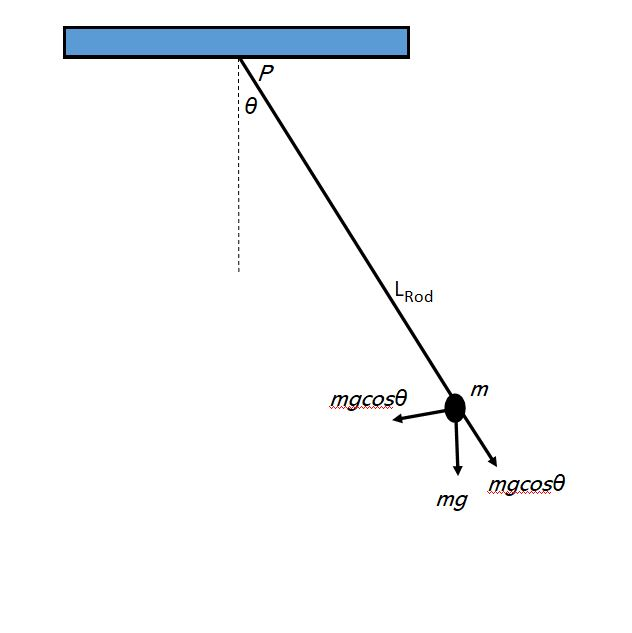
\includegraphics[width=0.7\textwidth]{../../../datafiles/DblPendulum/pendulum.png}
\caption{The physical system}
\label{Figure:Motion}
\end{center}
\end{figure}
\subsubsection{Goal Statements}
\label{Sec:GoalStmt}
Given the the mass length of the rod initial angle of the mass and the gravitational constant, the goal statements are:

\begin{itemize}
\item[motionMass:\phantomsection\label{motionMass}]{the Calculate the motion of the mass}
\end{itemize}
\subsection{Solution Characteristics Specification}
\label{Sec:SolCharSpec}
The instance models that govern Pendulum are presented in \hyperref[Sec:IMs]{Section: Instance Models}. The information to understand the meaning of the instance models and their derivation is also presented, so that the instance models can be verified.

\subsubsection{Assumptions}
\label{Sec:Assumps}
This section simplifies the original problem and helps in developing the theoretical models by filling in the missing information for the physical system. The assumptions refine the scope by providing more detail.

\begin{itemize}
\item[pend2DMotion:\phantomsection\label{pend2DMotion}]{The Pendulum motion is two-dimensional (2D).}
\item[cartCoord:\phantomsection\label{cartCoord}]{A Cartesian coordinate system is used}
\item[cartCoordRight:\phantomsection\label{cartCoordRight}]{The Cartesian coordinate system is right-handed where positive $x$-axis. and $y$-axis point right up}
\item[yAxisDir:\phantomsection\label{yAxisDir}]{The The direction of the $y$-axis is directed opposite to gravity.}
\item[startOrigin:\phantomsection\label{startOrigin}]{The Pendulum is attached to the origin.}
\end{itemize}
\subsubsection{Theoretical Models}
\label{Sec:TMs}
This section focuses on the general equations and laws that Pendulum is based on.

\vspace{\baselineskip}
\noindent
\begin{minipage}{\textwidth}
\begin{tabular}{>{\raggedright}p{0.13\textwidth}>{\raggedright\arraybackslash}p{0.82\textwidth}}
\toprule \textbf{Refname} & \textbf{TM:acceleration}
\phantomsection 
\label{TM:acceleration}
\\ \midrule \\
Label & Acceleration
        
\\ \midrule \\
Equation & \begin{displaymath}
           \mathbf{a}=\frac{\,d\mathbf{v}}{\,dt}
           \end{displaymath}
\\ \midrule \\
Description & \begin{symbDescription}
              \item{$\mathbf{a}$ is the acceleration ($\frac{\text{m}}{\text{s}^{2}}$)}
              \item{$t$ is the time (${\text{s}}$)}
              \item{$\mathbf{v}$ is the velocity ($\frac{\text{m}}{\text{s}}$)}
              \end{symbDescription}
\\ \midrule \\
Source & \cite{accelerationWiki} and \cite[(pg. 7)]{hibbeler2004}
         
\\ \midrule \\
RefBy & 
\\ \bottomrule
\end{tabular}
\end{minipage}
\vspace{\baselineskip}
\noindent
\begin{minipage}{\textwidth}
\begin{tabular}{>{\raggedright}p{0.13\textwidth}>{\raggedright\arraybackslash}p{0.82\textwidth}}
\toprule \textbf{Refname} & \textbf{TM:velocity}
\phantomsection 
\label{TM:velocity}
\\ \midrule \\
Label & Velocity
        
\\ \midrule \\
Equation & \begin{displaymath}
           \mathbf{v}=\frac{\,d\mathbf{p}}{\,dt}
           \end{displaymath}
\\ \midrule \\
Description & \begin{symbDescription}
              \item{$\mathbf{v}$ is the velocity ($\frac{\text{m}}{\text{s}}$)}
              \item{$t$ is the time (${\text{s}}$)}
              \item{$\mathbf{p}$ is the position (${\text{m}}$)}
              \end{symbDescription}
\\ \midrule \\
Source & \cite{velocityWiki} and \cite[(pg. 6)]{hibbeler2004}
         
\\ \midrule \\
RefBy & 
\\ \bottomrule
\end{tabular}
\end{minipage}
\vspace{\baselineskip}
\noindent
\begin{minipage}{\textwidth}
\begin{tabular}{>{\raggedright}p{0.13\textwidth}>{\raggedright\arraybackslash}p{0.82\textwidth}}
\toprule \textbf{Refname} & \textbf{TM:NewtonSecLawMot}
\phantomsection 
\label{TM:NewtonSecLawMot}
\\ \midrule \\
Label & Newton's second law of motion
        
\\ \midrule \\
Equation & \begin{displaymath}
           \mathbf{F}=m \mathbf{a}
           \end{displaymath}
\\ \midrule \\
Description & \begin{symbDescription}
              \item{$\mathbf{F}$ is the force (${\text{N}}$)}
              \item{$m$ is the mass (${\text{kg}}$)}
              \item{$\mathbf{a}$ is the acceleration ($\frac{\text{m}}{\text{s}^{2}}$)}
              \end{symbDescription}
\\ \midrule \\
Notes & The net force $\mathbf{F}$ on a body is proportional to the acceleration $\mathbf{a}$ of the body, where $m$ denotes the mass of the body as the constant of proportionality.
        
\\ \midrule \\
Source & --
         
\\ \midrule \\
RefBy & 
\\ \bottomrule
\end{tabular}
\end{minipage}
\subsubsection{General Definitions}
\label{Sec:GDs}
This section collects the laws and equations that will be used to build the instance models.

\vspace{\baselineskip}
\noindent
\begin{minipage}{\textwidth}
\begin{tabular}{>{\raggedright}p{0.13\textwidth}>{\raggedright\arraybackslash}p{0.82\textwidth}}
\toprule \textbf{Refname} & \textbf{GD:velocityIX}
\phantomsection 
\label{GD:velocityIX}
\\ \midrule \\
Label & $x$-component of the velocity
        
\\ \midrule \\
Units & $\frac{\text{m}}{\text{s}}$
        
\\ \midrule \\
Equation & \begin{displaymath}
           {v_{\text{x}}}=ω {L_{\text{rod}}} \cos\left(θ\right)
           \end{displaymath}
\\ \midrule \\
Description & \begin{symbDescription}
              \item{${v_{\text{x}}}$ is the $x$-component of velocity ($\frac{\text{m}}{\text{s}}$)}
              \item{$ω$ is the angular velocity ($\frac{\text{rad}}{\text{s}}$)}
              \item{${L_{\text{rod}}}$ is the length of rod (${\text{m}}$)}
              \item{$θ$ is the angle of pendulum (${{}^{\circ}}$)}
              \end{symbDescription}
\\ \midrule \\
Source & --
         
\\ \midrule \\
RefBy & 
\\ \bottomrule
\end{tabular}
\end{minipage}
\paragraph{Detailed derivation of $x$-component velocity:}
\label{GD:velocityIXDeriv}
\begin{displaymath}
{v_{\text{x}}}=ω {L_{\text{rod}}} \cos\left(θ\right)
\end{displaymath}
\vspace{\baselineskip}
\noindent
\begin{minipage}{\textwidth}
\begin{tabular}{>{\raggedright}p{0.13\textwidth}>{\raggedright\arraybackslash}p{0.82\textwidth}}
\toprule \textbf{Refname} & \textbf{GD:velocityIY}
\phantomsection 
\label{GD:velocityIY}
\\ \midrule \\
Label & $x$-component of the velocity
        
\\ \midrule \\
Units & $\frac{\text{m}}{\text{s}}$
        
\\ \midrule \\
Equation & \begin{displaymath}
           {v_{\text{y}}}=ω {L_{\text{rod}}} \cos\left(θ\right)
           \end{displaymath}
\\ \midrule \\
Description & \begin{symbDescription}
              \item{${v_{\text{y}}}$ is the $y$-component of velocity ($\frac{\text{m}}{\text{s}}$)}
              \item{$ω$ is the angular velocity ($\frac{\text{rad}}{\text{s}}$)}
              \item{${L_{\text{rod}}}$ is the length of rod (${\text{m}}$)}
              \item{$θ$ is the angle of pendulum (${{}^{\circ}}$)}
              \end{symbDescription}
\\ \midrule \\
Source & --
         
\\ \midrule \\
RefBy & 
\\ \bottomrule
\end{tabular}
\end{minipage}
\paragraph{Detailed derivation of $y$-component velocity:}
\label{GD:velocityIYDeriv}
\begin{displaymath}
{v_{\text{y}}}=ω {L_{\text{rod}}} \cos\left(θ\right)
\end{displaymath}
\vspace{\baselineskip}
\noindent
\begin{minipage}{\textwidth}
\begin{tabular}{>{\raggedright}p{0.13\textwidth}>{\raggedright\arraybackslash}p{0.82\textwidth}}
\toprule \textbf{Refname} & \textbf{GD:accelerationIX}
\phantomsection 
\label{GD:accelerationIX}
\\ \midrule \\
Label & $x$-component of acceleration
        
\\ \midrule \\
Units & $\frac{\text{m}}{\text{s}^{2}}$
        
\\ \midrule \\
Equation & \begin{displaymath}
           {a_{\text{x}}}=-ω {L_{\text{rod}}} \sin\left(θ\right)+α {L_{\text{rod}}} \cos\left(θ\right)
           \end{displaymath}
\\ \midrule \\
Description & \begin{symbDescription}
              \item{${a_{\text{x}}}$ is the $x$-component of acceleration ($\frac{\text{m}}{\text{s}^{2}}$)}
              \item{$ω$ is the angular velocity ($\frac{\text{rad}}{\text{s}}$)}
              \item{${L_{\text{rod}}}$ is the length of rod (${\text{m}}$)}
              \item{$θ$ is the angle of pendulum (${{}^{\circ}}$)}
              \item{$α$ is the angular acceleration ($\frac{\text{rad}}{\text{s}^{2}}$)}
              \end{symbDescription}
\\ \midrule \\
Source & --
         
\\ \midrule \\
RefBy & 
\\ \bottomrule
\end{tabular}
\end{minipage}
\paragraph{Detailed derivation of $x$-component acceleration:}
\label{GD:accelerationIXDeriv}
\begin{displaymath}
{a_{\text{x}}}=-ω {L_{\text{rod}}} \sin\left(θ\right)+α {L_{\text{rod}}} \cos\left(θ\right)
\end{displaymath}
\vspace{\baselineskip}
\noindent
\begin{minipage}{\textwidth}
\begin{tabular}{>{\raggedright}p{0.13\textwidth}>{\raggedright\arraybackslash}p{0.82\textwidth}}
\toprule \textbf{Refname} & \textbf{GD:accelerationIY}
\phantomsection 
\label{GD:accelerationIY}
\\ \midrule \\
Label & $y$-component of acceleration
        
\\ \midrule \\
Units & $\frac{\text{m}}{\text{s}^{2}}$
        
\\ \midrule \\
Equation & \begin{displaymath}
           {a_{\text{y}}}=ω {L_{\text{rod}}} \cos\left(θ\right)+α {L_{\text{rod}}} \sin\left(θ\right)
           \end{displaymath}
\\ \midrule \\
Description & \begin{symbDescription}
              \item{${a_{\text{y}}}$ is the $y$-component of acceleration ($\frac{\text{m}}{\text{s}^{2}}$)}
              \item{$ω$ is the angular velocity ($\frac{\text{rad}}{\text{s}}$)}
              \item{${L_{\text{rod}}}$ is the length of rod (${\text{m}}$)}
              \item{$θ$ is the angle of pendulum (${{}^{\circ}}$)}
              \item{$α$ is the angular acceleration ($\frac{\text{rad}}{\text{s}^{2}}$)}
              \end{symbDescription}
\\ \midrule \\
Source & --
         
\\ \midrule \\
RefBy & 
\\ \bottomrule
\end{tabular}
\end{minipage}
\paragraph{Detailed derivation of $x$-component acceleration:}
\label{GD:accelerationIYDeriv}
\begin{displaymath}
{a_{\text{y}}}=ω {L_{\text{rod}}} \cos\left(θ\right)+α {L_{\text{rod}}} \sin\left(θ\right)
\end{displaymath}
\subsubsection{Data Definitions}
\label{Sec:DDs}
This section collects and defines all the data needed to build the instance models.

\vspace{\baselineskip}
\noindent
\begin{minipage}{\textwidth}
\begin{tabular}{>{\raggedright}p{0.13\textwidth}>{\raggedright\arraybackslash}p{0.82\textwidth}}
\toprule \textbf{Refname} & \textbf{DD:positionIX}
\phantomsection 
\label{DD:positionIX}
\\ \midrule \\
Label & $x$-component of initial position
        
\\ \midrule \\
Symbol & ${{p_{\text{x}}}^{\text{i}}}$
         
\\ \midrule \\
Units & ${\text{m}}$
        
\\ \midrule \\
Equation & \begin{displaymath}
           {{p_{\text{x}}}^{\text{i}}}={L_{\text{rod}}} \sin\left(θ\right)
           \end{displaymath}
\\ \midrule \\
Description & \begin{symbDescription}
              \item{${{p_{\text{x}}}^{\text{i}}}$ is the $x$-component of initial position (${\text{m}}$)}
              \item{${L_{\text{rod}}}$ is the length of rod (${\text{m}}$)}
              \item{$θ$ is the angle of pendulum (${{}^{\circ}}$)}
              \end{symbDescription}
\\ \midrule \\
Notes & ${{p_{\text{x}}}^{\text{i}}}$ is the horizontal position
        
        ${{p_{\text{x}}}^{\text{i}}}$ is shown in \hyperref[Figure:Motion]{Fig:Motion}.
        
\\ \midrule \\
Source & --
         
\\ \midrule \\
RefBy & 
\\ \bottomrule
\end{tabular}
\end{minipage}

\vspace{\baselineskip}
\noindent
\begin{minipage}{\textwidth}
\begin{tabular}{>{\raggedright}p{0.13\textwidth}>{\raggedright\arraybackslash}p{0.82\textwidth}}
\toprule \textbf{Refname} & \textbf{DD:positionIY}
\phantomsection 
\label{DD:positionIY}
\\ \midrule \\
Label & $y$-component of initial position
        
\\ \midrule \\
Symbol & ${{p_{\text{y}}}^{\text{i}}}$
         
\\ \midrule \\
Units & ${\text{m}}$
        
\\ \midrule \\
Equation & \begin{displaymath}
           {{p_{\text{y}}}^{\text{i}}}={L_{\text{rod}}} \cos\left(θ\right)
           \end{displaymath}
\\ \midrule \\
Description & \begin{symbDescription}
              \item{${{p_{\text{y}}}^{\text{i}}}$ is the $y$-component of initial position (${\text{m}}$)}
              \item{${L_{\text{rod}}}$ is the length of rod (${\text{m}}$)}
              \item{$θ$ is the angle of pendulum (${{}^{\circ}}$)}
              \end{symbDescription}
\\ \midrule \\
Notes & ${{p_{\text{y}}}^{\text{i}}}$ is the vertical position
        
        ${{p_{\text{y}}}^{\text{i}}}$ is shown in \hyperref[Figure:Motion]{Fig:Motion}.
        
\\ \midrule \\
Source & --
         
\\ \midrule \\
RefBy & 
\\ \bottomrule
\end{tabular}
\end{minipage}

\section{Values of Auxiliary Constants}
\label{Sec:AuxConstants}
There are no auxiliary constants.

\section{References}
\label{Sec:References}
\begin{filecontents*}{bibfile.bib}
\end{filecontents*}
\nocite{*}
\bibstyle{ieeetr}
\printbibliography[heading=none]
\end{document}
